\chapter{Methodology and Experimental Design}
\label{ch:methodology}

\section{Study design and evidence levels}
The project follows an implementation-and-evaluation design. Its primary unit of analysis is an image, but its required unit of partitioning is the subject. Two evidence levels are distinguished:

\begin{description}
    \item[Engineering evidence] confirms that preprocessing, model loading, inference, metric computation, and artifact generation execute consistently.
    \item[Generalisation evidence] estimates performance on subjects independent of model development and requires verified subject-level separation, preserved provenance, and a frozen test set.
\end{description}

The current repository supports engineering evidence and a local patient-separated evaluation for the repaired BrEaST and OASBUD cohort. BUSI is excluded because the local derivative lacks traceable identifiers. The result remains local-cohort research evidence rather than external or clinical validation.

\section{Data sources and label mapping}
The local project combines organised copies of BUSI, OASBUD, and BrEaST. BUSI is a public B-mode image dataset with normal, benign, and malignant labels and lesion masks \citep{AlDhabyani2020}. OASBUD contains multiple views per lesion \citep{Piotrzkowska2017}. The BrEaST copy uses case identifiers and includes a small normal subset.

The configured task is binary: \texttt{benign} and \texttt{malignant}. Files in a \texttt{normal} directory are mapped to the non-malignant class by the loader. This makes the executable task consistent but collapses clinically different categories, so the decision must be reviewed and predeclared before a definitive experiment.

The validated loader finds the counts in Table~\ref{tab:local_counts}. Mask files are excluded from the image count; BUSI is retained for provenance context but excluded from validated training.

\begin{table}[htbp]
\centering
\caption{Images in the repaired validated local folders. BUSI is excluded because its patient identifiers are unavailable.}
\label{tab:local_counts}
\begin{tabular}{@{}lrrrr@{}}
\toprule
\textbf{Dataset} & \textbf{Training} & \textbf{Validation} & \textbf{Test} & \textbf{Total} \\ \midrule
BUSI & n/a & n/a & n/a & n/a \\
OASBUD & 138 & 30 & 30 & 198 \\
BrEaST & 164 & 33 & 32 & 229 \\ \midrule
Validated combined & 302 & 63 & 62 & 427 \\ \bottomrule
\end{tabular}
\end{table}

\section{Split-integrity audit}
The read-only audit enumerates eligible image files, derives subject identifiers where the naming convention permits, and records every partition associated with an identifier. For OASBUD it removes the view suffix; for BrEaST it uses the \texttt{caseNNN} prefix. The BUSI files in this local copy were renamed to generated sample identifiers, so patient separation cannot be reconstructed from filenames alone.

An audit passes only when every included dataset has verifiable identifiers and no identifier occurs in more than one partition. The repaired OASBUD and BrEaST folders pass this check. BUSI remains unverifiable and is excluded from the validated run. The training entry point stops by default if a configured dataset fails; an \texttt{-{}-allow-unaudited-data} override exists solely for explicitly provisional engineering runs and is recorded in the checkpoint through the audit status.

The \texttt{rebuild\_subject\_splits.py} utility copies grouped source files into deterministic subject partitions and writes a manifest. Copying rather than moving preserves the legacy source dataset. The generated manifest and audit report should be retained with run metadata, subject to dataset licensing constraints.

\section{Preprocessing pipeline}
All training, evaluation, command-line prediction, and API routes call the same preprocessing implementation. Images are decoded to RGB, optionally enhanced with CLAHE, transformed according to a selected geometric strategy, converted to tensors, and normalised with ImageNet channel statistics for the transfer-learning backbones.

Figure~\ref{fig:pipeline_overview} summarises the implementation path. The diagram is a software view of the experiment: the audit determines which files can enter the validated cohort, preprocessing defines the tensor presented to the model, and the evaluator writes the evidence consumed by the report and dashboard. Keeping these stages explicit reduces the risk that a browser demonstration silently uses a different transformation from the reported checkpoint.

\begin{figure}[htbp]
    \centering
    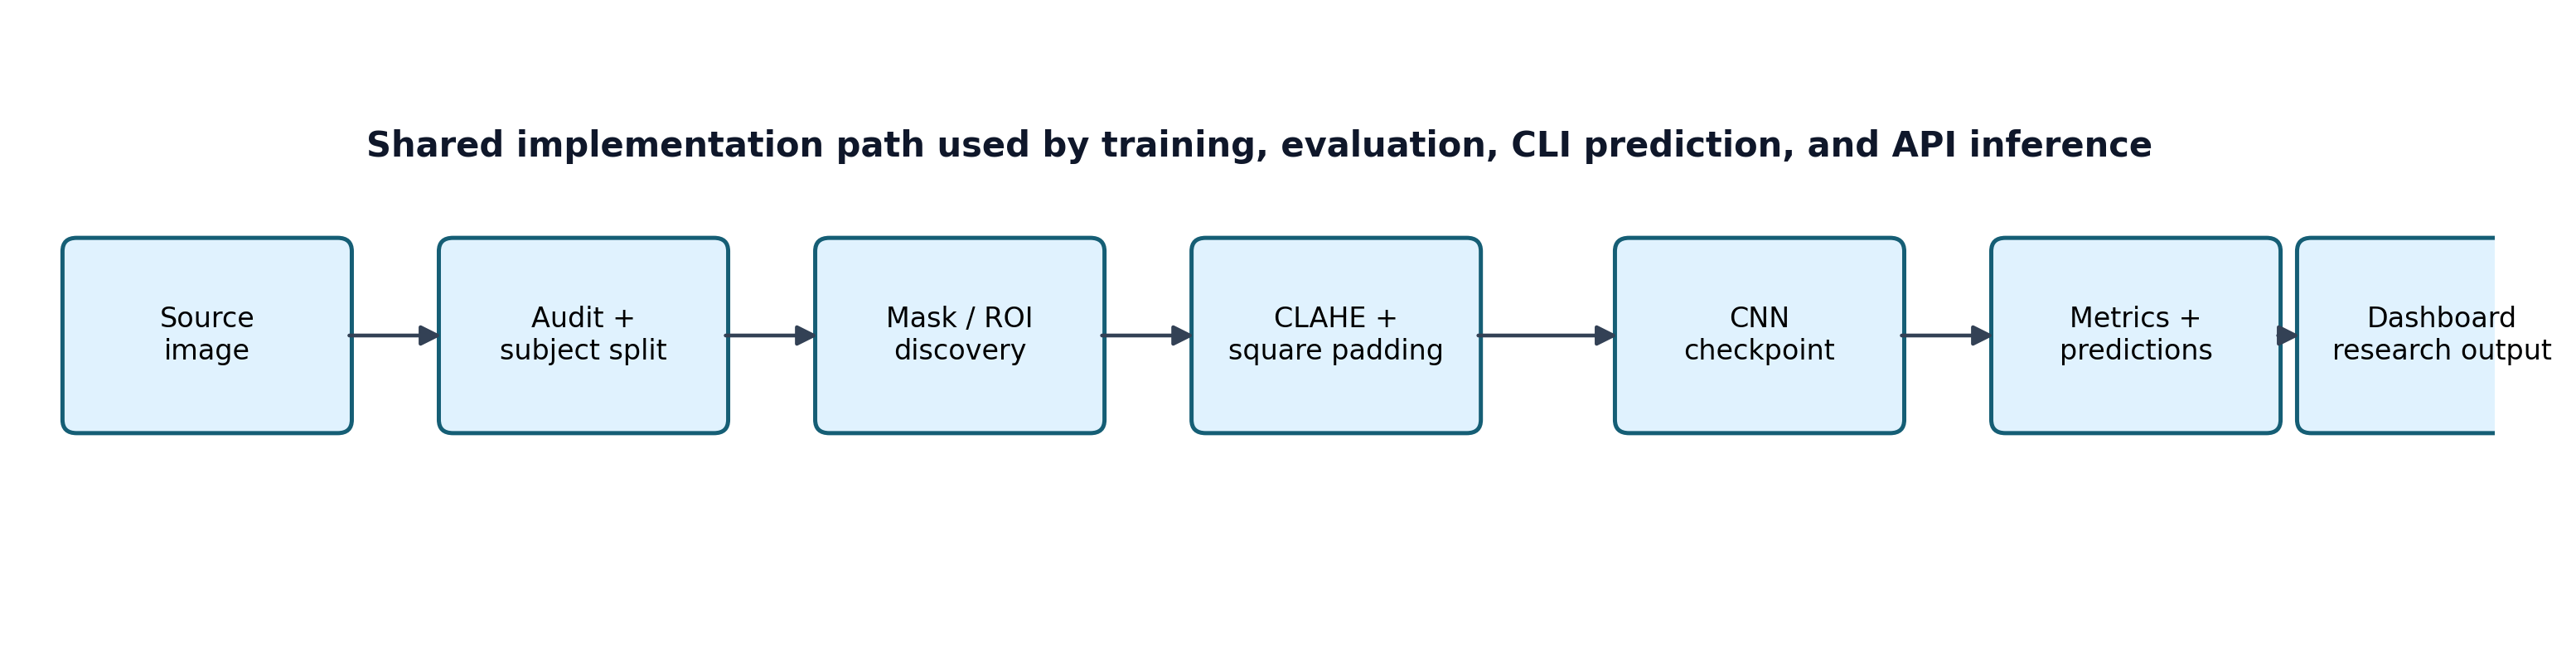
\includegraphics[width=0.92\textwidth]{figures/fig7_pipeline_overview.png}
    \caption{Implementation path shared by training, evaluation, command-line prediction, and API inference.}
    \label{fig:pipeline_overview}
\end{figure}

\subsection{CLAHE}
The image is converted from RGB to LAB. CLAHE is applied only to the luminance channel using OpenCV with clip limit 2.0 and a $16\times16$ tile grid; the result is then converted back to RGB. The operation can be disabled through configuration or request parameters.

\subsection{Mask discovery and region selection}
The loader recognises paired masks ending in \path{_mask.png}, \path{_tumor.png}, or \path{_lesion_mask.png}. When a non-empty mask is available, the inclusive lesion bounding box is expanded by a 20\% width and height margin, clipped to the image boundaries, and extracted. When no mask is available, the implementation uses the central 80\% of the image before margin expansion. This fallback is deterministic but is not lesion localisation and is documented as such.

\subsection{Square padding}
For a crop of height $h_c$ and width $w_c$, let
\begin{equation}
d=\max(h_c,w_c).
\end{equation}
The vertical and horizontal padding are
\begin{align}
p_t &= \left\lfloor\frac{d-h_c}{2}\right\rfloor,
&p_b &= d-h_c-p_t,\\
p_l &= \left\lfloor\frac{d-w_c}{2}\right\rfloor,
&p_r &= d-w_c-p_l.
\end{align}
OpenCV \texttt{BORDER\_REFLECT\_101} fills the boundary, after which the square is resized to $224\times224$ pixels with bicubic interpolation. Because both output axes scale from side $d$, the final resize is isotropic. Direct resize and centre crop are implemented as comparator strategies.

\subsection{Augmentation}
Training uses random horizontal flips and rotations up to $15^{\circ}$. Vertical flips are intentionally excluded because the depth axis has acquisition meaning in ultrasound. Validation and test transforms contain no random augmentation.

\section{Model architectures}
Three architectures share a two-class output contract:

\begin{itemize}
    \item \textbf{EfficientNet-B0} initialised from torchvision ImageNet weights, with its classifier replaced by dropout and a two-output linear layer \citep{Tan2019};
    \item \textbf{ResNet-50} initialised from torchvision ImageNet weights, with its fully connected layer replaced by dropout and a two-output linear layer \citep{He2016}; and
    \item \textbf{Custom CNN} with four convolutional stages, batch normalisation, ReLU, max pooling, adaptive average pooling, dropout, and a two-output linear layer.
\end{itemize}

Transfer learning is used only during training. Evaluation reconstructs the architecture without downloading pretrained weights and loads the stored state dictionary.

Figure~\ref{fig:architecture_overview} shows the implementation-level comparison. The blocks are schematic rather than parameter-count diagrams; their purpose is to show the different representation pathways that lead to the same two-class output. EfficientNet-B0 and ResNet-50 use ImageNet initialisation, while the custom CNN learns its convolutional representation from the project data. All three are evaluated through the same loader and metric writer.

\begin{figure}[htbp]
    \centering
    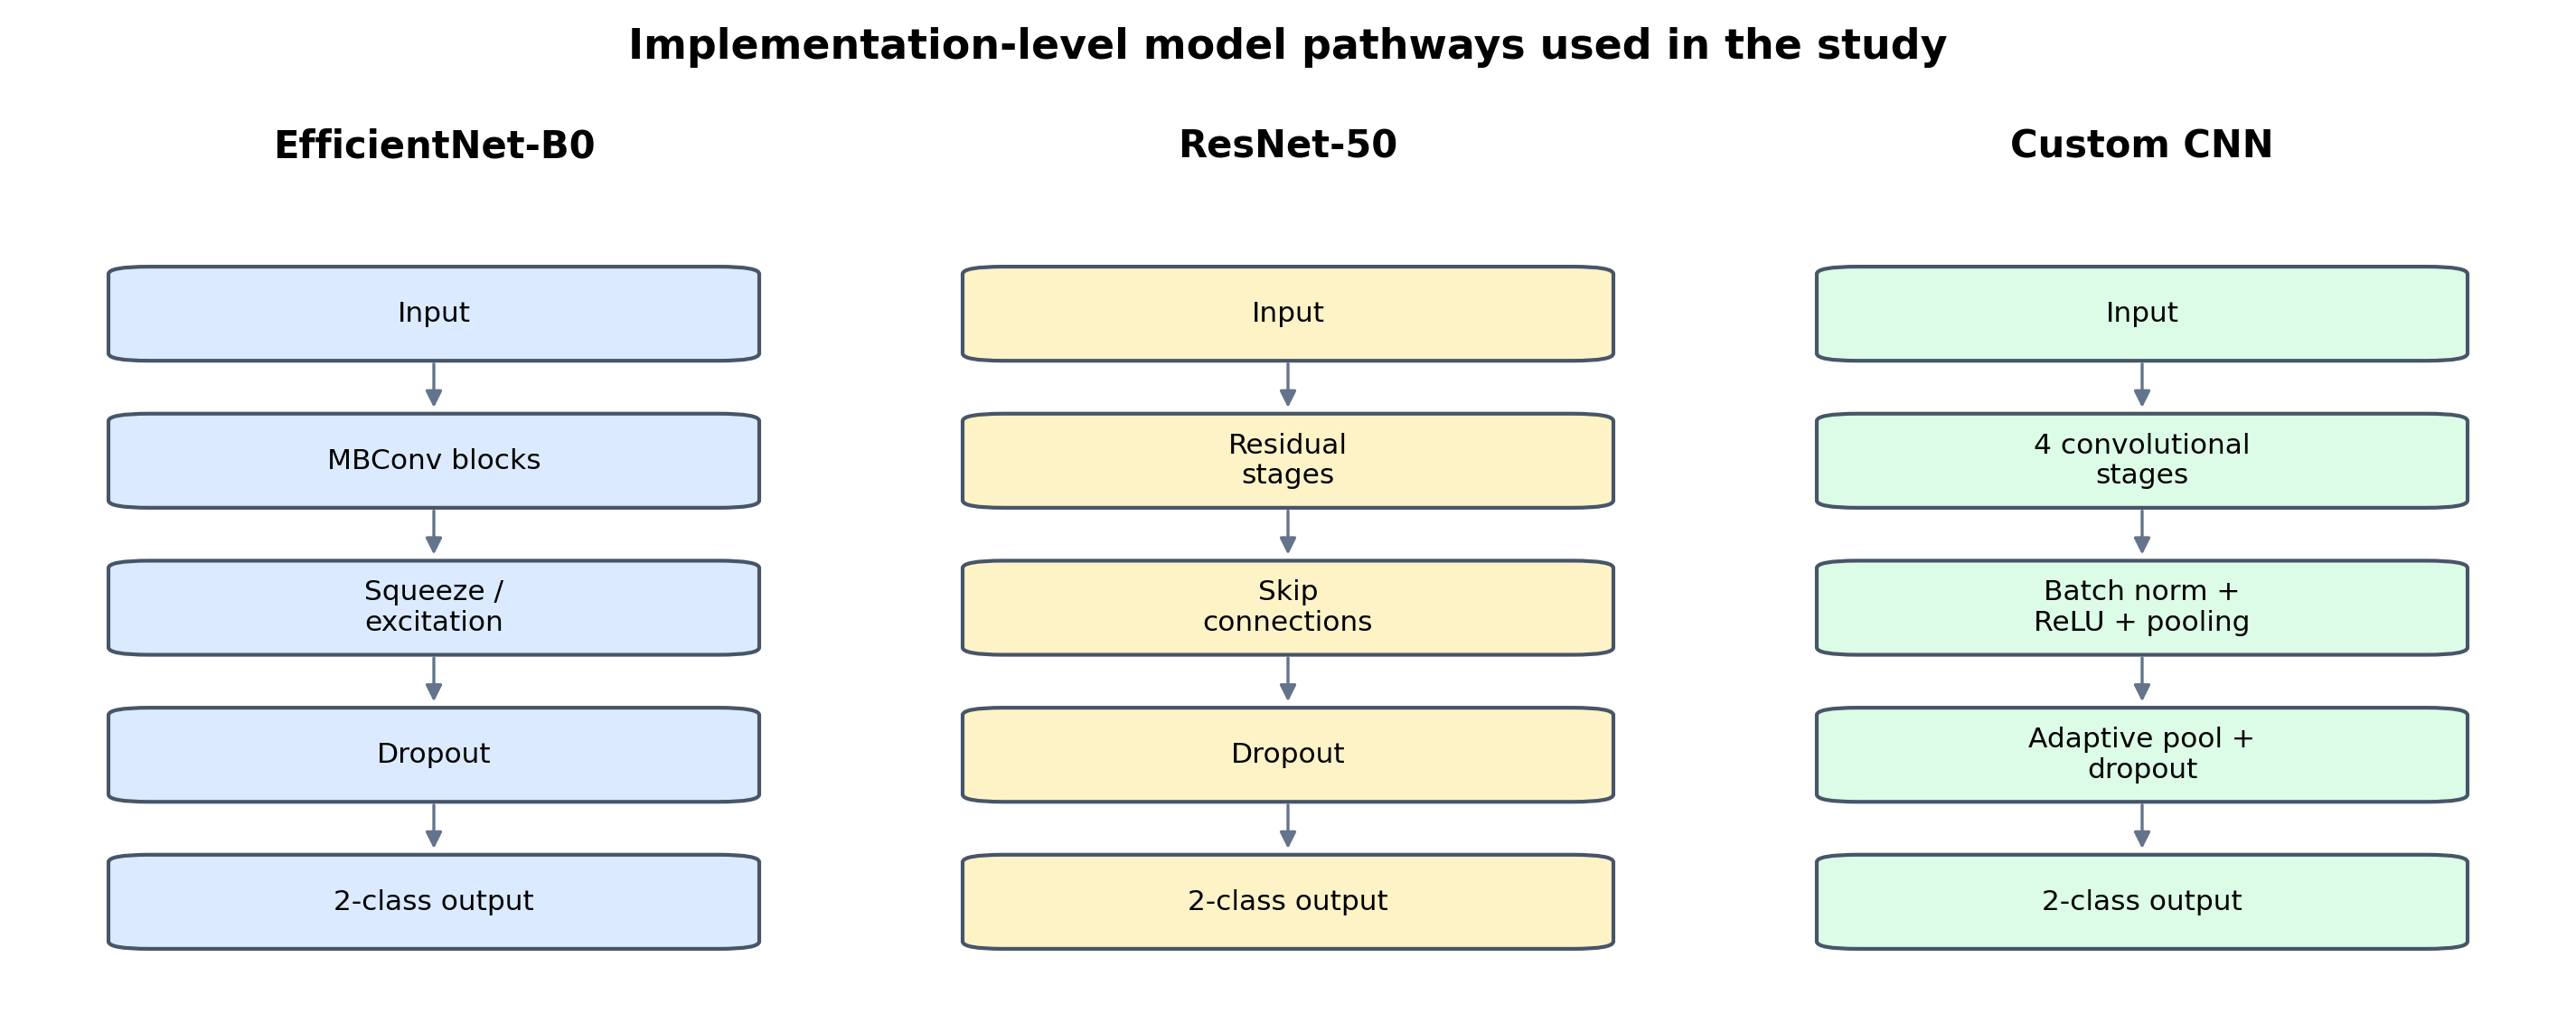
\includegraphics[width=0.96\textwidth]{figures/fig8_architecture_overview.png}
    \caption{Schematic implementation pathways for the three model families.}
    \label{fig:architecture_overview}
\end{figure}

\section{Optimisation and reproducibility controls}
The default optimisation configuration uses class-weighted cross-entropy, AdamW with learning rate $10^{-4}$ and weight decay $10^{-4}$, cosine annealing, batch size 16, up to 25 epochs, and early stopping after five validation epochs without loss improvement. Class weights are computed from the training directory counts as
\begin{equation}
w_c=\frac{N}{K N_c},
\end{equation}
where $N$ is the training size, $K$ is the number of classes, and $N_c$ is the count for class $c$.

The training command accepts a seed, defaulting to 42, and seeds Python, NumPy, PyTorch, and CUDA where available. Each best-loss checkpoint stores the architecture, epoch, optimiser state, validation loss and accuracy, class names, seed, learning rate, batch size, requested epoch budget, dataset-combination flag, crop strategy, CLAHE flag, creation time, and data-audit status.

Exact bitwise reproducibility can still depend on hardware, library versions, and non-deterministic kernels. A final run should therefore record the environment lock, device, repository revision, and checksums in addition to the checkpoint metadata.

\section{Evaluation protocol}
The evaluator loads a named checkpoint and processes validation or test data without random augmentation. For each sample it records the relative path, true class, predicted class, and malignant-class probability. It then writes:

\begin{itemize}
    \item \texttt{predictions.csv}, the per-image evidence table;
    \item \texttt{metrics.json}, including accuracy, macro precision, macro recall, macro F1, ROC-AUC, confusion matrix, preprocessing configuration, generation time, audit status, and audit checksum;
    \item \texttt{confusion\_matrix.png}; and
    \item \texttt{roc\_curve.png}.
\end{itemize}

Accuracy is
\begin{equation}
\operatorname{Accuracy}=\frac{TP+TN}{TP+TN+FP+FN},
\end{equation}
and class F1 is
\begin{equation}
F1=2\frac{\operatorname{Precision}\times\operatorname{Recall}}{\operatorname{Precision}+\operatorname{Recall}}.
\end{equation}
Macro metrics average class-level values equally. ROC-AUC is calculated from malignant-class probabilities for this binary task. The current post-hoc analysis adds confidence intervals and a descriptive reliability diagram from the stored test probabilities. A definitive experiment would predeclare exclusions and missing-data handling, fit any calibration method on validation data, and preserve the test set for one final evaluation.

\section{Web research demonstration}
FastAPI serves model inference and a static interface. Upload validation limits files to recognised image formats and 20 MB. The client exposes the selected preprocessing configuration, probability vector, Grad-CAM overlay, image-quality heuristics, batch outputs, and controlled seeded perturbations. It also reads the evaluator's metrics file rather than embedding benchmark values.

The interface does not assign a diagnosis, BI-RADS category, clinical priority, or management recommendation. Its report text and batch labels explicitly identify outputs as research-only. Ground truth is accepted only when supplied by the dataset endpoint or the user; it is never inferred from a filename.

Figure~\ref{fig:web_interface} shows the implemented single-image workspace after loading a labelled example. The persistent navigation separates prediction, noise, batch, evidence, dataset, and documentation tasks. The header keeps the selected model and preprocessing controls visible, while the main panel places the source image beside the Grad-CAM inspection layer. A yellow evidence banner tells the viewer that the results are provisional. This layout makes the experimental configuration and evidence status harder to overlook during a demonstration.

\begin{figure}[htbp]
    \centering
    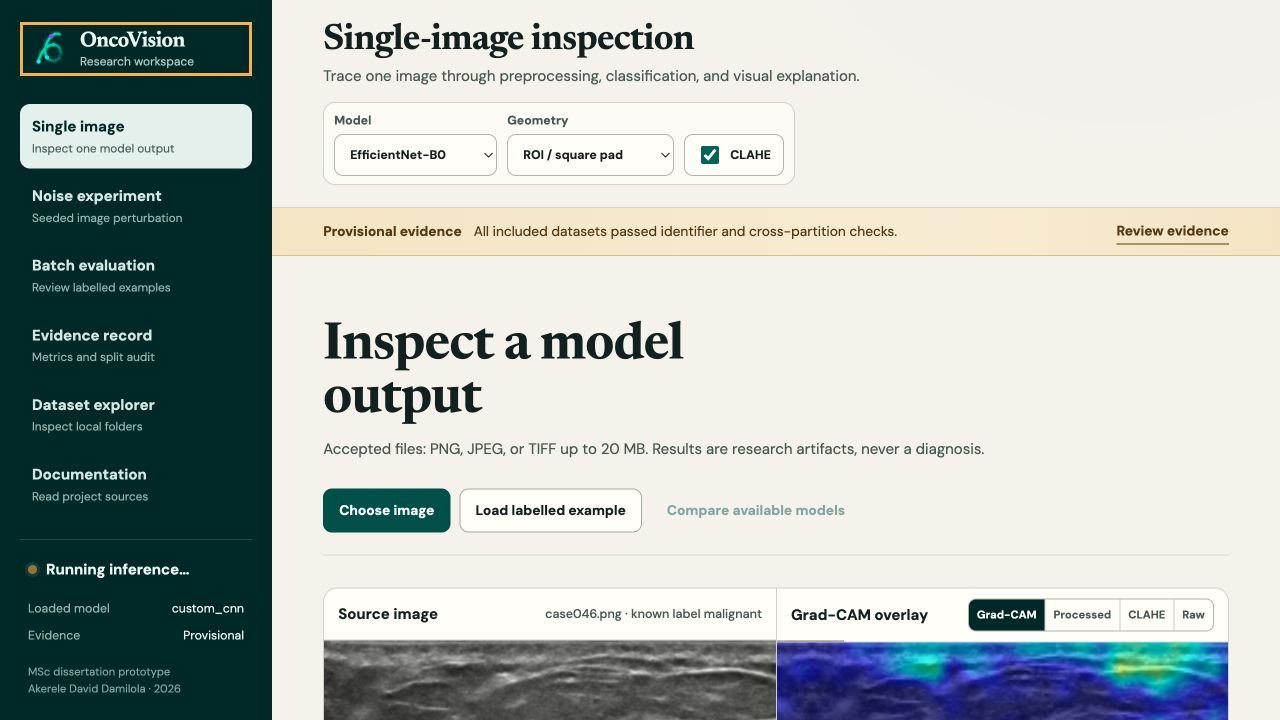
\includegraphics[width=0.98\textwidth]{figures/fig11_web_interface.png}
    \caption{Implemented OncoVision research dashboard showing the single-image inspection workspace, model and preprocessing controls, source image, and Grad-CAM layer. The interface identifies the evidence as provisional and the output as a research artefact.}
    \label{fig:web_interface}
\end{figure}

Figure~\ref{fig:web_interface_tour} records the complete browser-facing workflow. The single-image page supports case inspection; the noise page applies a seeded perturbation to one image; the batch page processes labelled research examples; the evidence page reads generated metrics and the split audit; the dataset page exposes folder contents with a provenance warning; and the documentation page states appropriate and unsupported use before presenting the project record. These pages share one model and preprocessing configuration bar so a demonstrator can see the active settings.

\begin{figure}[htbp]
    \centering
    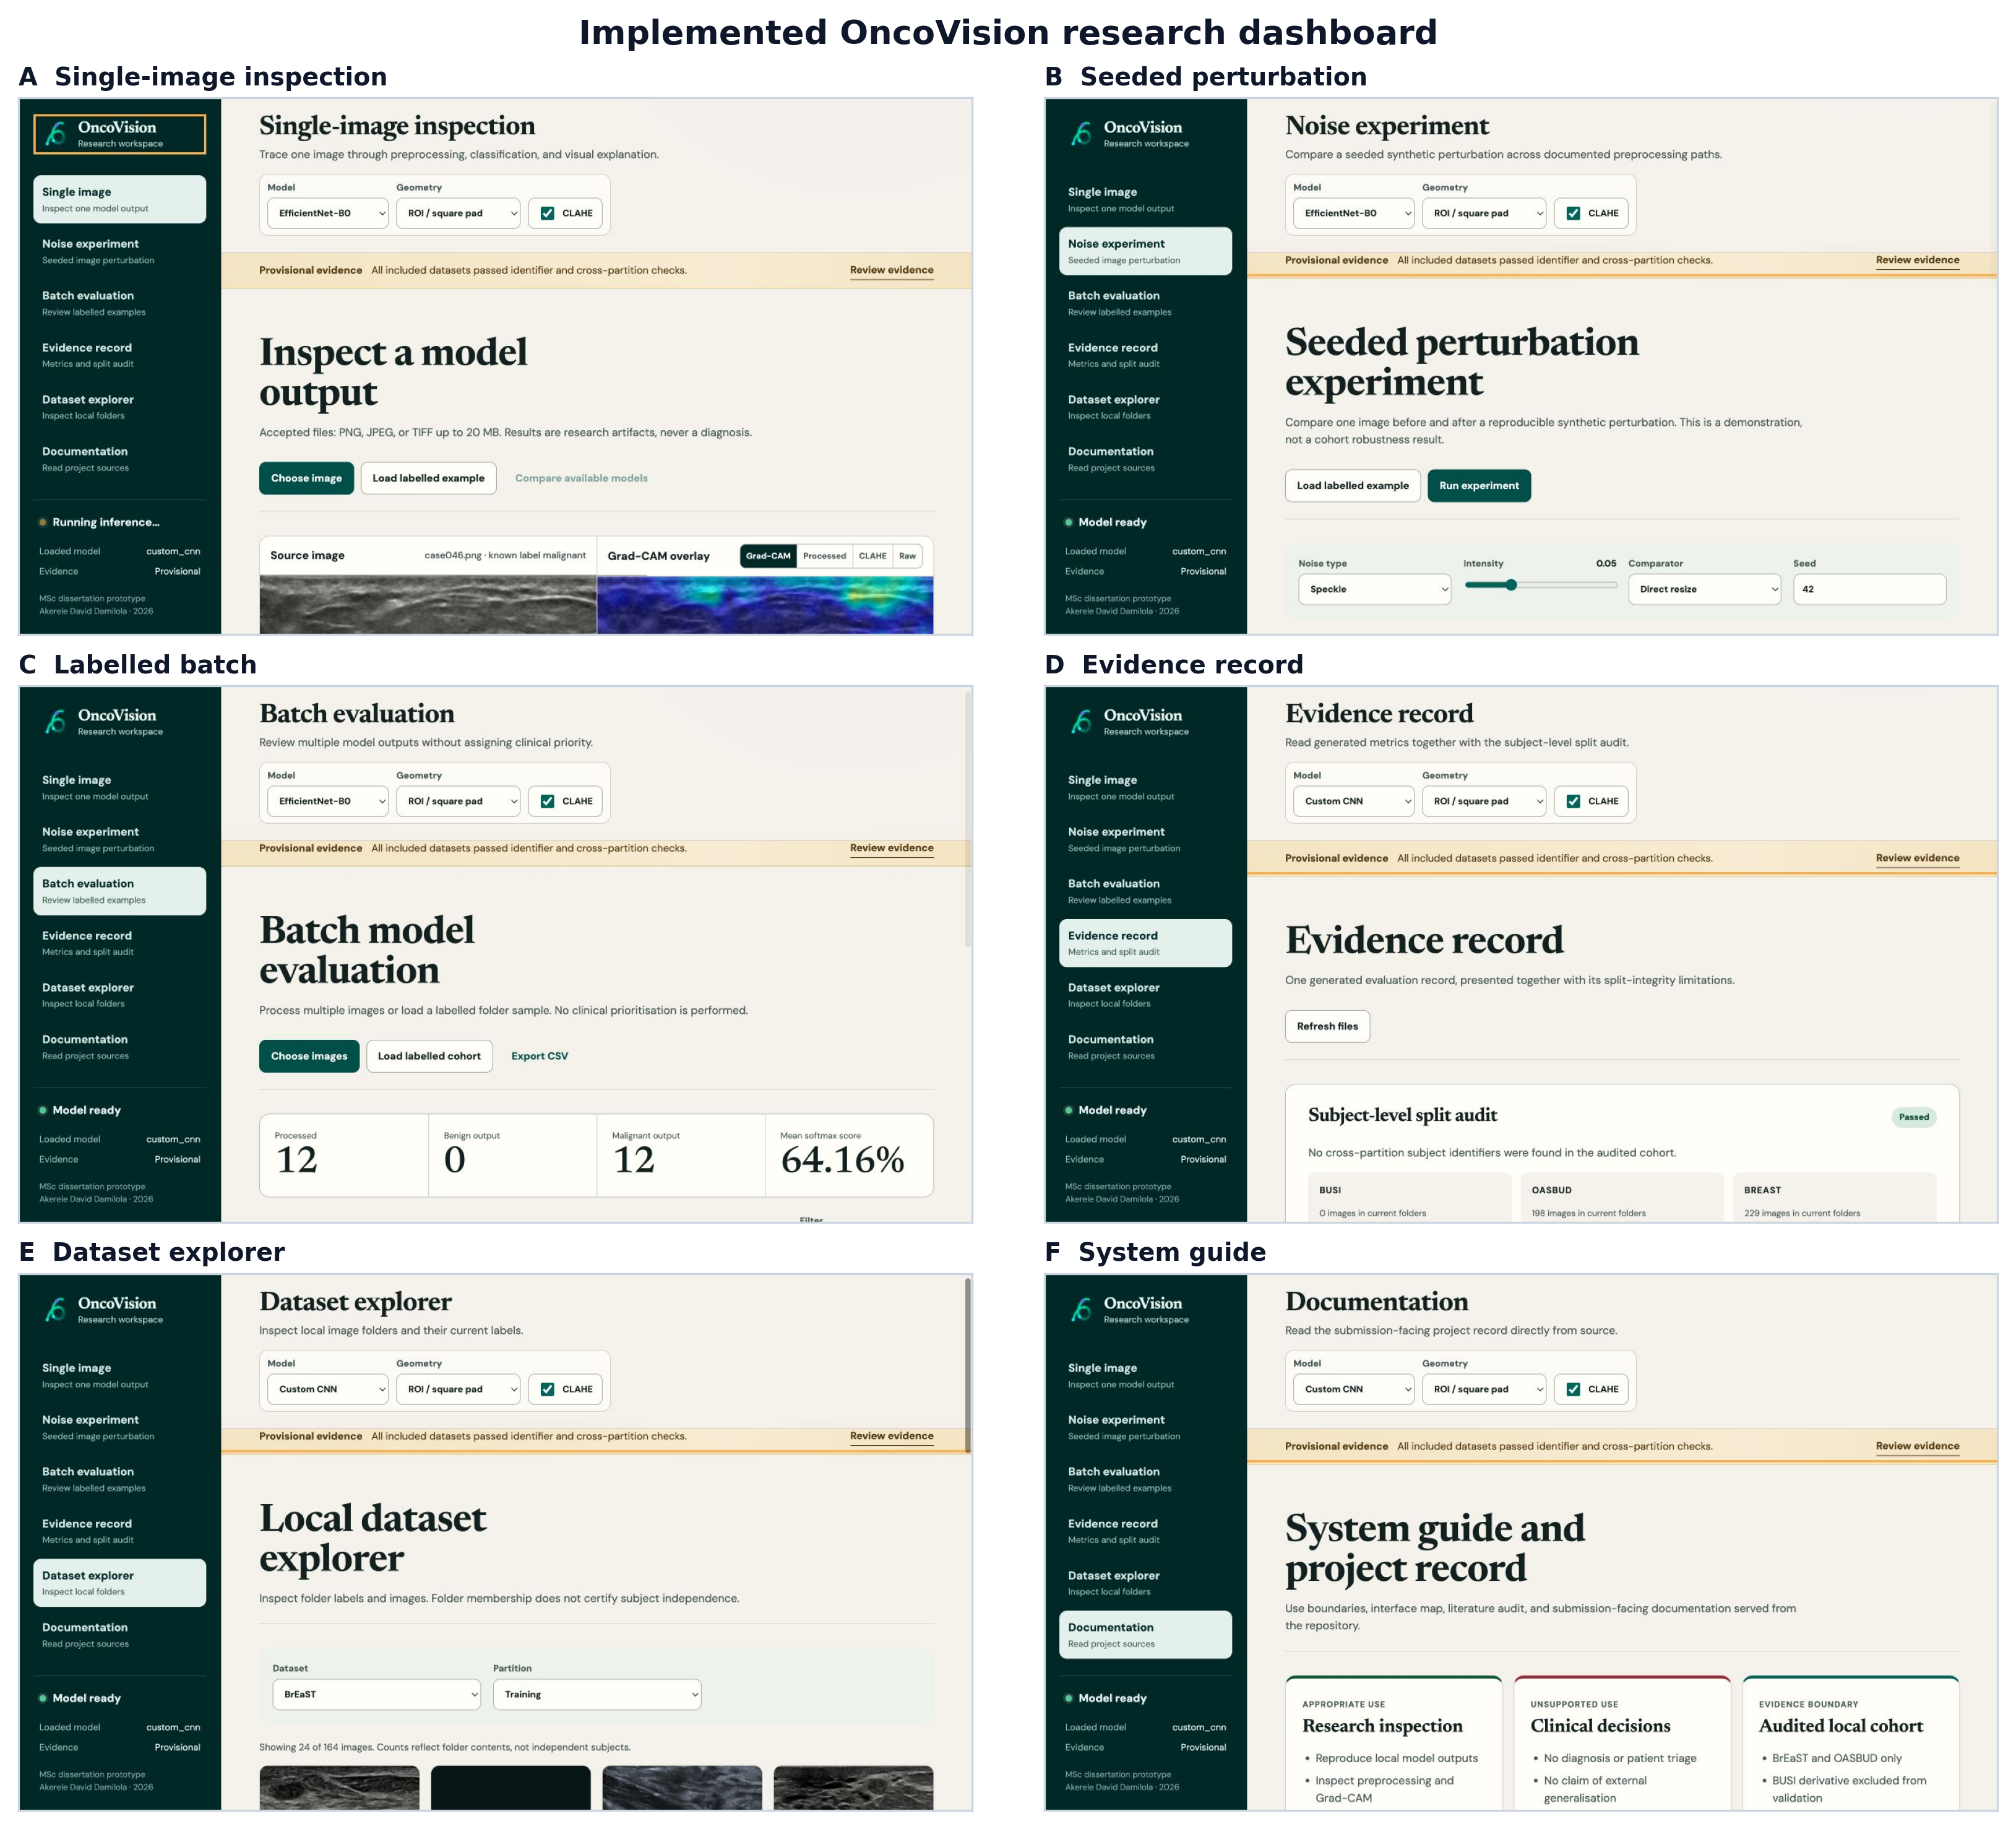
\includegraphics[width=0.98\textwidth]{figures/fig14_web_interface_tour.png}
    \caption{Browser-verified tour of the implemented dashboard. Panels A to F show single-image inspection, a seeded perturbation demonstration, labelled batch output, generated evidence, the local dataset explorer, and the research-use guide. The screens are documentation of the software, not additional model-performance evidence.}
    \label{fig:web_interface_tour}
\end{figure}

\section{Definitive experiment specification}
Before comparative claims are reported, the following sequence is required:

\begin{enumerate}
    \item recover original identifiers and document licences, versions, exclusions, and label mapping;
    \item assign all images, views, and masks from one subject to exactly one partition;
    \item freeze the test manifest before model selection;
    \item select preprocessing and hyperparameters using training and validation data only;
    \item train each comparator across predeclared seeds and equal tuning budgets;
    \item evaluate locked checkpoints once on the untouched test subjects;
    \item publish per-image predictions, aggregate metrics with uncertainty, audit outputs, and failure analysis; and
    \item regenerate all dissertation tables and figures directly from those artifacts.
\end{enumerate}

This sequence converts the implemented framework into a valid generalisation study while preserving the distinction between exploratory development and final evidence.

\section{Operational data curation}
The audit is intentionally read-only during ordinary evaluation. It enumerates eligible files, applies dataset-specific identifier parsers, and records every partition associated with each identifier. A report that only counts files can appear balanced while hiding duplicate subjects; a report that only checks folder names can miss a duplicated identifier under a different filename. The audit output is therefore a table of observations, not merely a pass/fail flag.

For the current cohort, the BrEaST parser retains the case prefix and the OASBUD parser removes the view suffix. These identifiers are used for grouping and audit purposes, not as model features. The manifest should be treated as sensitive research metadata. It may be committed in an anonymised form when the dataset licence permits, while a private mapping to source records is retained by the research team. This supports reproducibility without unnecessarily redistributing patient-linked information.

Label mapping deserves the same attention as grouping. The binary task treats benign and malignant as the output classes and maps a normal directory to the non-malignant class. That convention makes the loader compatible with heterogeneous folders, but it combines a normal screening appearance with a benign lesion. A definitive study could use three classes, exclude normals, or define a clinically motivated two-class question. The choice should be made before inspecting test results because it changes the meaning of precision, recall, and error severity.

\section{Preprocessing as a versioned transform}
The shared preprocessing function is a contract between the dataset and every consumer of a checkpoint. It should be possible to take one source image, apply the stored configuration, and obtain the same tensor during training, evaluation, command-line prediction, and web inference. Configuration values such as image size, CLAHE state, crop strategy, padding mode, normalisation constants, and augmentation policy are therefore recorded rather than inferred from the interface.

The transform is deterministic after random training augmentation has been separated from validation and test. This makes failure analysis practical: an investigator can reproduce the pixels that generated a probability, compare them with the original image, and test a proposed change without adding a new random factor. It also makes the dashboard honest. A selected direct-resize option must change the operation used by the evaluator, not merely change a label in the browser.

The fallback crop is particularly important to document. When a mask is absent, the implementation uses a central region as a conservative placeholder. The lesion may be elsewhere, so the crop is not a lesion localisation method. It keeps the research pipeline executable while making missing annotation visible. A production-oriented implementation would require a validated detector, an explicit no-mask policy, or human review instead of silently treating the centre as ground truth.

\section{Model comparison and training controls}
The three architectures represent different capacity and inductive-bias choices. EfficientNet-B0 offers a compact transfer-learning backbone; ResNet-50 provides a deeper residual comparator; and the custom CNN supplies a small from-scratch baseline. A comparison is meaningful only when the surrounding conditions are aligned. The same subject partitions, input size, class definition, early-stopping rule, and evaluation script should be used for every model. If one network receives more tuning or a different augmentation policy, the result is a comparison of complete recipes rather than architectures.

Class-weighted cross-entropy gives a rare class more influence, but it does not create new clinical information and can increase variance when counts are small. Weights must therefore be computed from the training partition only. Validation and test labels must not affect the loss, threshold, or checkpoint selection. This separation is recorded in training metadata and should be checked whenever a run is reproduced.

The seed is a reproducibility control, not a guarantee of certainty. It fixes intended pseudo-random streams, yet hardware, library versions, and parallel kernels may still change final weights. The recommended record includes Python and PyTorch versions, device type, repository revision, source-data checksum, and checkpoint hash. These details make it possible to explain a small rerun difference rather than treating it as an unexplained modelling improvement.

\section{Metric interpretation}
Accuracy is intuitive but can conceal class imbalance. Macro recall gives each class equal weight and is useful when errors in either class matter. ROC-AUC measures ranking across thresholds, whereas a deployed decision requires one operating threshold. Calibration measures whether predicted probabilities correspond to observed frequencies; a model can have reasonable AUC and still be overconfident. The evaluator therefore stores probabilities and per-image predictions so that additional metrics can be calculated without retraining.

Uncertainty intervals are particularly important for a small test partition. A bootstrap interval is not a substitute for a larger sample or external site, but it communicates how much a point estimate would move under resampling. It should be described as an uncertainty summary for sampled images, not a guarantee about future patients. A final protocol should predeclare the interval method, number of resamples, and treatment of degenerate class samples.

\section{Web interface and software verification}
The web application is a research instrument for making the pipeline inspectable. Upload validation limits input type and size, while the API exposes preprocessing choice and separates the raw model prediction from the display-level abstention label. Batch mode reads the same model and transformation as single-image inference. The metrics view reads generated evaluator artefacts instead of embedding a manually typed score, reducing the chance that dashboard and dissertation diverge.

Software tests check contracts that would otherwise fail silently: processed dimensions, paired-mask discovery, audit status in outputs, and the research-only API wording. These tests do not prove medical validity. They provide a minimum guard against accidental changes to the data path while scientific questions remain under study. A seeded brightness, contrast, or noise change is likewise a demonstration until it is applied to a held-out set and reported with prediction-level metrics and uncertainty.

\section{Run management and artefact lineage}
Each experiment should be treated as a small bundle rather than a single checkpoint. The bundle contains the configuration, audit report, manifest reference, model state, metrics, predictions, plots, and environment information. Naming the bundle with a run identifier prevents a later evaluation from overwriting the files used to write the dissertation. It also makes it possible to compare a provisional run with a corrected run without relying on memory.

The evaluator's checksum is a lightweight lineage mechanism. It does not prove that the underlying public dataset has not changed, but it records which audit output was associated with a result. In a final submission, the checksum should be accompanied by a repository revision and a data-release identifier. When licences prevent redistribution of images, these metadata still allow an authorised collaborator with the same source archive to verify the run.

\section{Reproducible training sequence}
A complete training sequence begins with a clean audit, writes the selected dataset list, sets the seed, constructs the dataloaders, and records the model and optimiser configuration before the first update. During training, validation loss and accuracy are written at every epoch so that early stopping can be inspected. The selected checkpoint is the one defined by the stopping rule, not the last file written to disk. Evaluation then loads that checkpoint with random augmentation disabled.

This sequence avoids a common ambiguity in student projects, where a reported model may have been trained for one number of epochs but evaluated from another saved state. It also separates model selection from test measurement. If a later change improves validation loss, the old test result remains intact and can be compared as a previous run rather than silently replaced.

\section{Ethical handling of uncertainty}
The interface wording is part of the methodology because users interpret labels in context. Research-only language, visible preprocessing settings, and the abstention state reduce the risk that a demonstration is mistaken for a medical recommendation. The application should also make it easy to inspect the original image and generated overlays rather than presenting a single coloured badge as if it were a diagnosis. These are modest human-factors controls, but they are appropriate for the scope of the project.

An ethical presentation also avoids implying that a low-confidence image is unimportant. Abstention means that the model's output is not decisive under the configured rule; it does not mean that the underlying case is benign or safe to ignore. Documentation should say this explicitly and should discourage use outside the research context.
